\documentclass[a4paper,12pt]{article}
\usepackage[english]{babel}
\usepackage[utf8]{inputenc}
\usepackage{libertine}
\usepackage{libertinust1math}
\usepackage[T1]{fontenc}
\usepackage{inconsolata}

\usepackage[top=1.5cm, bottom=2.5cm, left=1cm, right=1cm]{geometry}

\usepackage{datetime}
\newdateformat{monthyeardate}{%
  \monthname[\THEMONTH], \THEYEAR}

\usepackage{subcaption}

% Math packages
\usepackage{mathtools}
\usepackage{amsmath}
\usepackage{amsfonts}
\usepackage{amssymb}
\DeclarePairedDelimiter{\ceil}{\lceil}{\rceil}

\usepackage{enumitem}
\usepackage{algorithm}
\usepackage{algpseudocode}

\usepackage{listings}

\usepackage{makecell}

\usepackage[hidelinks]{hyperref}

\title{Mobile and Social Sensing Systems}
\author{Francesco Barbarulo, Giovan Battista Rolandi}
\date{\monthyeardate\today}

\begin{document}
\pagenumbering{roman}

\maketitle
\abstract{The aim of these notes is to give some pills of every argument for the oral test. We have assumed that the reader has attended the lessons because these notes, by themselves, are not sufficient to have a global and profound knowledge.

We wish you good luck!}

\tableofcontents

\newpage

\pagenumbering{arabic}

\section{Introduction}

Mobile computing relys on the ability to use devices \textit{non-physically connected} and \textit{context-aware}. Mobility can be:
\begin{itemize}
  \item \textbf{physical}: hardware actually changes its physical position;
  \item \textbf{logical}: applications and data may need to be moved for design reasons.
\end{itemize}
These devices must keep computinal and communicaiton capabilities paying attention to energy comsumption because of their battery-powered nature.

\section{Localization systems}
Localization systems consist of two main blocks:
\begin{enumerate}[label=(\roman*)]
	\item Set of deployed nodes with different \textit{states}:
		\begin{itemize}
		 	\item \textbf{beacon} (\textit{landmarks} or \textit{anchors}): already know their locations through a manual configuration or through GPS reading;
		  	\item \textbf{unknown} (\textit{targets}): do not have any information about their geographic locations;
		  	\item \textbf{settled}: targets nodes that has determined or estimated their locations.
		\end{itemize}
	\item Localization algorithm:
		\begin{itemize}
			\item GPS not longer used in CPS for cost and energy constraints;
			\item \textbf{GPS-free} techniques exploit the sensing and the wireless communication capabilities of CPS components.
		\end{itemize}
\end{enumerate}

\subsection{Topology}
The topology of a localization algorithm refers to \textit{where} and \textit{how} the location of a given node is calculated:

\begin{itemize}
	\item \textbf{Centralized localizaiton}: a central device estimates the location of unknown nodes based on the signal measurements forwarded by anchors;
	\item \textbf{Localized localization}: each object estimates its location using the collected signal measurements and location information of the anchor nodes in its neighbourhood.
\end{itemize}

We can distinguish four different system topologies for localization systems, as shown in Figure~\ref{fig:topology}.
\begin{figure}
	\centering
  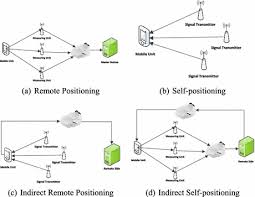
\includegraphics[width=0.6\textwidth]{img/topology}
  \caption{\label{fig:topology}Taxonomy of localization systems topology}
\end{figure}

\subsection{Coordinate System}
\begin{itemize}
  \item \textbf{Physical}: locations are represented as a point in a 2D/3D coordinate system;
  \item \textbf{Symbolic}: locations are expressed as logical positions’ information;
  \item \textbf{Absolute}: locations are expressed as unique coordinate values making reference to \textit{anchor} nodes that know their positions;
  \item \textbf{Relative}: locations are determined relatively to other nodes with no reference to absolute anchors.
\end{itemize}

\subsection{Communication paradigm}
\begin{itemize}
  \item \textbf{Non-cooperative}: the communication is restricted between unknown nodes and anchors (\textit{high density} of anchors or \textit{long-range anchor transmissions} are needed);
  \item \textbf{Cooperative}: allows communication between unknown nodes (more \textit{processing} is required);
  \item \textbf{Opportunistic}: exploits interactions between nodes that occasionally pass each other in their proximity (efficient \textit{node discovery} and \textit{data exchange}).
\end{itemize}

\subsection{Performance metrics}
\begin{itemize}
  \item \textbf{Accuracy}: mean (Euclidean) distance error between the estimated location and the true location;
  \item \textbf{Precision}: variation over many algorithm trials, CDF of distance error;
  \item \textbf{Complexity}: hardware and/or software;
  \item \textbf{Robustness}: behavior under unwanted conditions;
  \item \textbf{Scalability}: geographical and density;
  \item \textbf{Cost}
\end{itemize}

\subsection{Category}
The catogery of the localization technique pertains to how the location of a node is calculated depending on whether they are based on distance measurement or not. The two main categories are: \textit{range-based} and \textit{range-free}. 

Note that all the presented techniques are classified as \textit{anchor-based} schemes, assuming the existence of nodes with known positions.

\subsubsection{Range-based}
Range-based (or distance-based) techniques rely on the computation of distances between the target node and the anchor nodes to infer the position of a target node using \textit{lateration} techniques.

Location discovery consists of two phases:
\begin{enumerate}
  \item \textbf{Ranging phase} (or measuring distance): each node estimates its distance or angle from neighbors based on information contained in \textit{beacon} messages.
  The main three distance measuring methods are: 

  \begin{enumerate}[label=(\roman*)]
    \item \textit{Received Signal Strength (RSS)} estimates the distance from some set of neighbors using the attenuation of emitted signal strength. In free space, the RSS varies as the inverse square of the distance $d$ between the transmitter and the receiver:

    \begin{equation}
    P_r(d) = \frac{P_t G_t G_r \lambda^2}{(4\pi)^2 d^2}
    \end{equation}

    where $ P_r $ and $ P_t $ are respectively the reception and transmission power, $ G $ is the antenna gain, $ \lambda $ is constant and $ d $ is the distance between transmitter and receiver. Unfortunately, RSS is unreliable as it gets affected by the random multi-path effect.

    The parameters employed in these models are \textit{site-specific} and an empirical model is derived by obtaining a least square fit for each power level:

    \begin{equation}
    P_{RSSI} = \frac{X}{d^n}
    \end{equation}

    \item \textit{Time of Arrival} consists in calculating the one way propagation time of radio signals (RF) between two \textbf{synchronized} nodes. This time is proportional to the distance between transreceivers and is given by Eq.~\ref{eq:toa}:

    \begin{equation}
    d = c_r \times (t_1 - t_0)
    \label{eq:toa}
    \end{equation}

    This method of RF signals is usually inappropriate for WSNs because of short distances and inaccurate time synchronization of sensor nodes.

    \begin{figure}[b]
    \centering
    \begin{subfigure}{.5\textwidth}
      \centering
      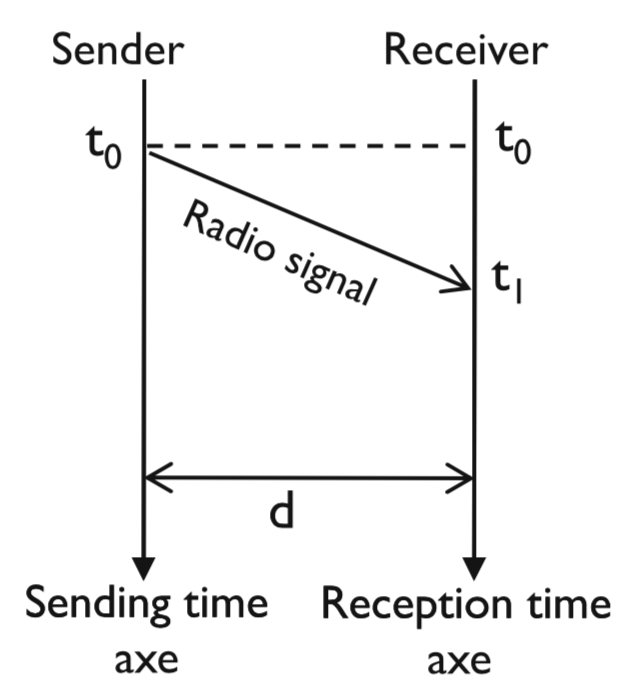
\includegraphics[width=.4\linewidth]{img/toa}
      \caption{Time of Arrival}
    \end{subfigure}%
    \begin{subfigure}{.5\textwidth}
      \centering
      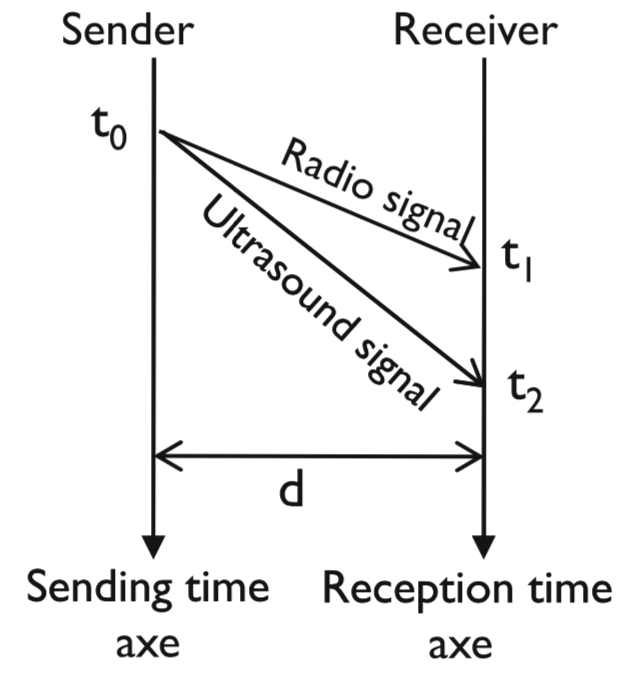
\includegraphics[width=.4\linewidth]{img/tdoa}
      \caption{Time Difference of Arrival}
    \end{subfigure}
    \caption{Time-based localization techiques}
    \end{figure}

    The TOA method can be used with Ultra-wideband (UWB) radio with which high accuracy can be achieved regardless the clock resolution thanks to the small propagation speed of ultrasound radios. This method is referred to as \textit{Time Difference of Arrival} (TDoA) and is based on the measurement of the time difference of the propagation of radio signals and ultrasound signals. When a node (anchor) simultaneously sends an RF signal and an ultrasound signal, the receiver (target) considers the arrival time of the (faster) radio signal as a time reference and uses the arrival time of the (slower) ultrasound radio to calculate the delay between the two signals. The distance is calculated according to Eq.~\ref{eq:tdoa}:

    \begin{equation}
    d = \frac{c_r \times c_u \times (t_2 - t_1)}{c_r - c_u}
    \label{eq:tdoa}
    \end{equation}

    where $c_r$ and $c_u$ are respectively the propagation speed of both radio and ultrasound signals, while $t_1$ and $t_2$ are their reception times at the receiver level.

    The TDOA method has the advantage to provide much better accuracy than RSS-based methods and it does not suffer from the need of explicit synchronization between nodes. However, it presents the drawback of requiring additional and more complex hardware with two different transceivers, which would have a negative impact on the cost.

    \item \textit{Angle of Arrival} relies on computing the angle by two lines connecting the unknown node with two anchor nodes. This technique relies on the use of directional antennas that can rotate on their axis or an array of antennas. For locating the unknown node at least three anchor nodes in 3D space and two anchor nodes in 2D space are needed.

    The advantage of AoA is that it does not require time sinchronization but on the other hand it requires vomplex and expensive hardware.
  \end{enumerate}

  \item \textbf{Estimation phase} (or combining distance): nodes use range information and anchors' locations to estimate their positions. In this phase some \textit{geometric geolocation techniques} are used:

  \begin{figure}[b]
    \centering
    \begin{subfigure}{.5\textwidth}
      \centering
      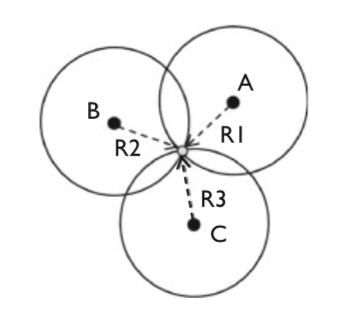
\includegraphics[width=.4\linewidth]{img/noise-free-lateration}
      \caption{with noise-free measurements}
    \end{subfigure}%
    \begin{subfigure}{.5\textwidth}
      \centering
      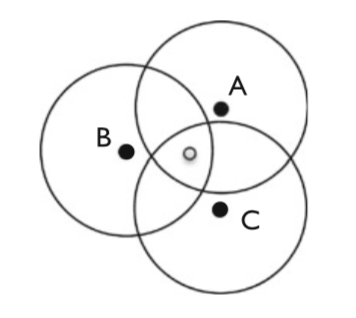
\includegraphics[width=.4\linewidth]{img/lateration}
      \caption{with noisy measurements}
    \end{subfigure}
    \caption{Trilateration technique}
  \end{figure}

  \begin{enumerate}[label=(\roman*)]
    \item \textit{Lateration/Trilateration} is the technique that uses distance information from anchor nodes to locate a target. In a 2D space, lateration involves the determination of the location of an unknown node as the intersection point of three circles centered in three non-collinear anchors (A, B and C), given that distances R1, R2 and R3 (i.e. circle radii) between the node and anchors are known. This technique is referred to as \textit{trilateration}. In a 3D space, there is a need of at least four anchor nodes to determine the location of a target node.
    \item \textit{Triangulation} is based on angle measurements to estimate the location of an unknown node.
    \item \textit{Multi-lateration} takes in consideration more than the minimum number of required anchor nodes.
  \end{enumerate}
\end{enumerate}

\paragraph{Limitations}
Some of the analyzed range-based localization techniques are based on assumptions that do not always hold or are impractical such as circular radio range, symmetric radio connectivity, lack of obstructions, clear line-of-sight.

\subsubsection{Range-free}
Range-free methods do not rely on distance or angle estimation in localization. They rather use proximity or connectivity information to devise the location of the target.

Anchor-based range-free localization techniques can be classified as:
\begin{enumerate}[label=(\alph*)]
  \item \textit{Area-based approaches} estimate the position of the target as a particular point in the polygon formed by the anchor nodes. Two main methods are proposed:
  \begin{enumerate}[label=(\roman*)]
    \item \textit{Centroid} consists in computing the location of the target as the \textit{centroid} point, defined as the barycenter of a set of anchors, as shown in Figure~\ref{fig:centroid}. In the most general form, assuming $n$ anchor nodes $A_i$ with coordinates $(X_i, Y_i )$ are detected by the target node (through beacon listening), the latter calculates its
    coordinate $(X_G, Y_G)$ such that:

    \begin{equation}
    (X_G, Y_G) = (\frac{\sum_{i=1}^n(X_i)}{n}, \frac{\sum_{i=1}^n(Y_i)}{n})
    \end{equation}

    Note that the more the number of anchors we have, the more accuracy we will obtain.

    \begin{figure}[t]
      \centering
      \begin{subfigure}{.5\textwidth}
        \centering
        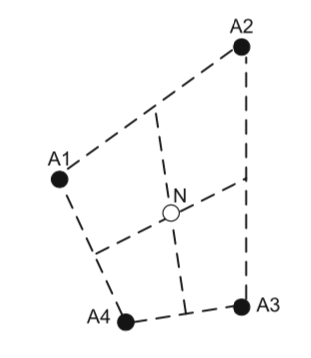
\includegraphics[width=.4\linewidth]{img/centroid}
        \caption{\label{fig:centroid}Centroid}
      \end{subfigure}%
      \begin{subfigure}{.5\textwidth}
        \centering
        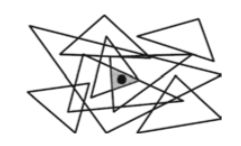
\includegraphics[width=.4\linewidth]{img/apit}
        \caption{\label{fig:apit}APIT}
      \end{subfigure}
      \caption{Area-base localization techniques}
    \end{figure}

    \item \textit{Approximate Point-In-Triangle (APIT)} assumes that the location of the target is the center of gravity of a certain triangle, which is defined as the intersection of triangles formed by anchors in which the target node resides, as illustrated in Figure~\ref{fig:apit}.

    The idea is to divide the environment into triangular regions, testing whether the target is inside a given triangle or not. The center of gravity of the triangles' intersection will represent the estimation target position.

    The main challenge in this technique is to determine whether the target is inside or outside a certain triangle. The idea, illustrated in Figure~\ref{fig:pit-test}, referred to as \textit{perfect PIT} and relies on checking the existence of a direction such that if the target moves according to that direction, it will simultaneously get further/closer to all triangle points, i.e. anchors.
    Two major handicaps hinder the practicability of this approach in real-world. First, nodes typically do not have the ability to recognize the direction without moving. Second, it is not possible to perform an exhaustive test covering all possible directions in which the target may move to. To solve both problems, an approximation has been proposed and whose idea is to use neighborhood information, exchanged via beaconing, to emulate the node movement in the Perfect PIT test as shown in Figure~\ref{fig:apit-test}:
    \begin{enumerate}[label=\arabic*.]
      \item The target node asks its neighbors for their distances to three corner anchors;
      \item The target compares its distance to these three corner anchors against those of its neighbors;
      \item If there exists at least one anchor such that it is further from or closer to all corner anchors than the target, then the latter considers itself as being outside the triangle.
    \end{enumerate}

    \begin{figure}[H]
      \centering
      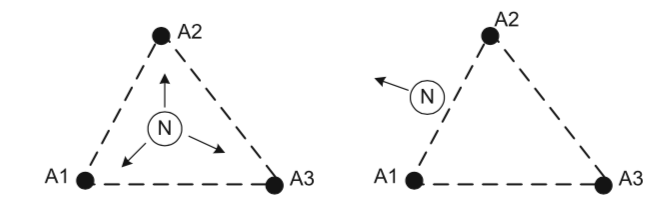
\includegraphics[width=0.7\textwidth]{img/pit-test}
      \caption{\label{fig:pit-test}Possible cases in point-in-triangle test. $N$ denotes the target node, and $A_i$ denotes the $i$-th anchor. The \textit{left figure} shows that if the target $N$ is inside the triangle moves in any direction, it will get close to some anchors and far from others. In the \textit{right figure}, if the target node $N$ is outside the triangle moves in the indicated direction, it will get far to all anchors at the same time.}
    \end{figure}

    \begin{figure}[h]
      \centering
      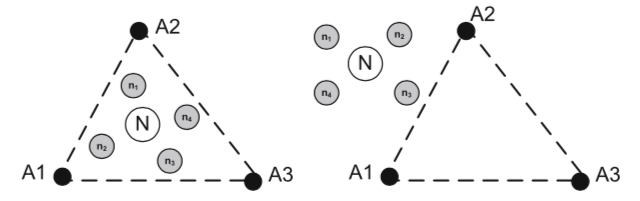
\includegraphics[width=0.7\textwidth]{img/apit-test}
      \caption{\label{fig:apit-test}Possible cases in approximate point-in-triangle test. $N$ denotes the target node, and $A_i$ denotes the $i$-th anchor. The \textit{left figure} shows that if the target $N$ is inside the triangle, none of its neighbors is either close to or far from all anchors. In the \textit{right figure}, if the target node $N$ is outside the triangle, its neighbor $n_1$ indicates that is it further to all anchors than it.}
    \end{figure}

   % TODO -- Relative Distance Estimation, Error scenarios, Pros and Cons

  \end{enumerate}
  \item \textit{Multi-hop localization approaches} are used when a target is not in communication range with at least three anchor nodes because of the limitation of the transmission power. In this case the idea consists in flooding the network such that each anchor independently broadcasts a \textit{beacon}, embedding its location and a hop-counter field initially set to one and increased in each new hop. Then, each target node identifies the shortest-path to each anchor node and tries to estimate its distance to it. One of the \textit{distance propagation methods} is:
  \begin{enumerate}[label=(\roman*)]
    \item \textit{DV-Hop}: the idea is to compute the number of hops between any two anchors $(A_i, A_j)$ and each anchor estimates the average 1-hop distance by dividing the sum of its distance to other anchors (\textit{physical distance}) by the sum of hop counts to those anchors (\textit{logical distance}). The process consists in three steps:
    \begin{enumerate}[label=\arabic*.]
    	\item \textit{Node update phase}: when a target node $N_i$ receives a beacon from an anchor, it maintains the record $(X_i, Y_i, h_i)$ for each anchor $A_i$, where $(X_i, Y_i)$ represents the location of the anchor, and $h_i$, the number of hops from $N_i$ to that anchor $A_i$.
    	\item \textit{1-hop distance estimation phase}: when an anchor node receives the locations and hop counts to the other anchors, it calculates the estimated average 1-hop distance, refereed to as \textit{correction factor} $c_i$, expressed as follows:
    	\begin{equation}
    	c_i = \frac{\sum(\sqrt{(x_i - x_j)^2 + (y_i - y_j)^2})}{\sum{(h_i)}}
    	\end{equation}
    	Then the anchor floods the network with the estimated 1-hop distance. A node that recives a correction, forwards it and then stops forwarding subsequent corrections.
    	\item \textit{Target node localization}: each target uses the correction sent from the \textbf{closest} anchor as the estimated 1-hop distance. It then multiplies the 1-hop distance by the hop counts to the other anchors to estimate its physical distance to them. After getting distance estimates to at least three anchors, a target can use trilateration to approximate its location.
    \end{enumerate}
    An example is shown in Figure~\ref{fig:dv-hop}.

    \begin{figure}[t]
      \centering
      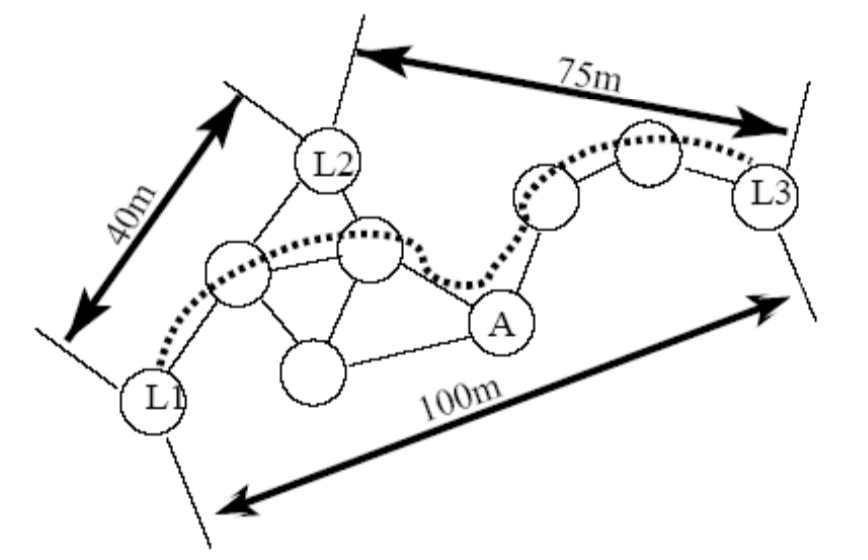
\includegraphics[width=0.4\textwidth]{img/dv-hop}
      \caption{\label{fig:dv-hop}DV-Hop example with anchor nodes $L_1$, $L_2$, $L_3$ and target node $A$. $c_1 = \frac{100+40}{6+2} = 17.5$, $c_2 = \frac{40+75}{2+5} = 16.42$, $c_3 = \frac{75+100}{6+5} = 15.90$. Target $A$ gets the correction from the closest anchor $L_2$ and computes the distance to $L_1 = 3 \times 16.42$, $L_2 = 2 \times 16.42$, $L_3 = 3 \times 16.42$.}
    \end{figure}
  \end{enumerate}
\end{enumerate}

\newpage

\section{Publish-Subscribe Pattern}
The Public-Subscribe pattern is a messaging pattern where sender of messages, called \textit{publishers}, do not program the messages to be sent directly to specific receivers, called \textit{subscribers}, but instead categorize published messages into classes without knowledge of which subscribers, if any, tehre may be.

Similarly, \textit{subscribers} express interest in one or more classes and only receive messages that are of interest, without knowledge of which publishers, if any, they are. The process of selecting messages for reception and processing is called \textbf{filtering}:
\begin{itemize}
  \item in a \textbf{topic-based} system messages are published to \textit{topics} and subscribers will receive only messages published to topics to which they subscribe.
  \item in a \textbf{content-based} system messages are only delivered to a subscriber if the attributes or content of those messages matches constraints defined by the subscriber.
\end{itemize}

Many solutions have been proposed for implementing the Publish-Subscribe system shown in Figure~\ref{fig:ps-problem}:
\begin{itemize}
  \item \textbf{client-server} solution is simple but not scalable, resulting in an overload on the server which is a single point of failure.
  \item \textbf{peer-to-peer (P2P)} architecture is a distributed system with a large number of heterogeneous and unreliable nodes, but it discloses the \textit{lookup} problem, i.e. how to know where the \textit{repository} node is. Three possible approach have been proposed:
  \begin{itemize}
    \item \textbf{centralized} approach based on a \textit{coordinator} node which must maintain $O(N)$ status and represents a single point of failure;
    \item \textbf{flooding} approach which foresees $O(N)$ messages per lookup;
    \item \textbf{DHT} approach which foresees $O(\log(N))$ messages per lookup, but building and maintenance of \textbf{routing tables} is needed.
  \end{itemize}
\end{itemize}

\begin{figure}[b!]
  \centering
  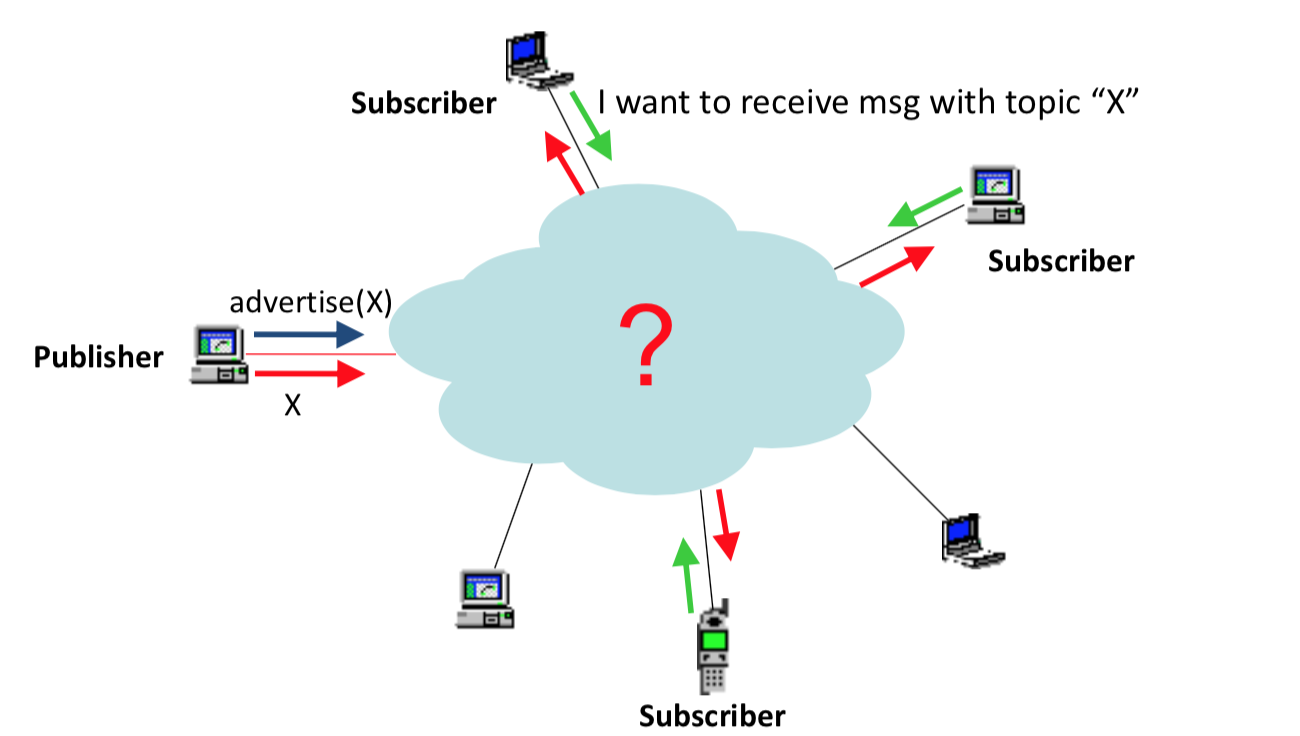
\includegraphics[width=0.8\textwidth]{img/ps-problem}
  \caption{\label{fig:ps-problem} Publish-Subscribe problem}
\end{figure}


\subsection{Distributed Hash Table (DHT)}
A Distributed Hash Table (DHT) described in Figure~\ref{fig:dht} is a distributed system that provides a \textbf{lookup} service similar to a hash table: $(key, value)$ pairs are stored in a DHT, and any participating node can efficiently retrieve the value associated with a given key. 

The main advantage of a DHT is that nodes can be added/removed with minimum work around re-distributing keys. Keys are unique identifiers which map to particular values, which in turn can be anything from addresses, to documents, to arbitrary data. Responsibility for maintaining the mapping from keys to values is distributed among the nodes, in such a way that a change in the set of participants causes a minimal amount of disruption. This allows a DHT to scale to extremely large numbers of nodes and to handle continual node arrivals, departures, and failures.

\begin{figure}[t]
  \centering
  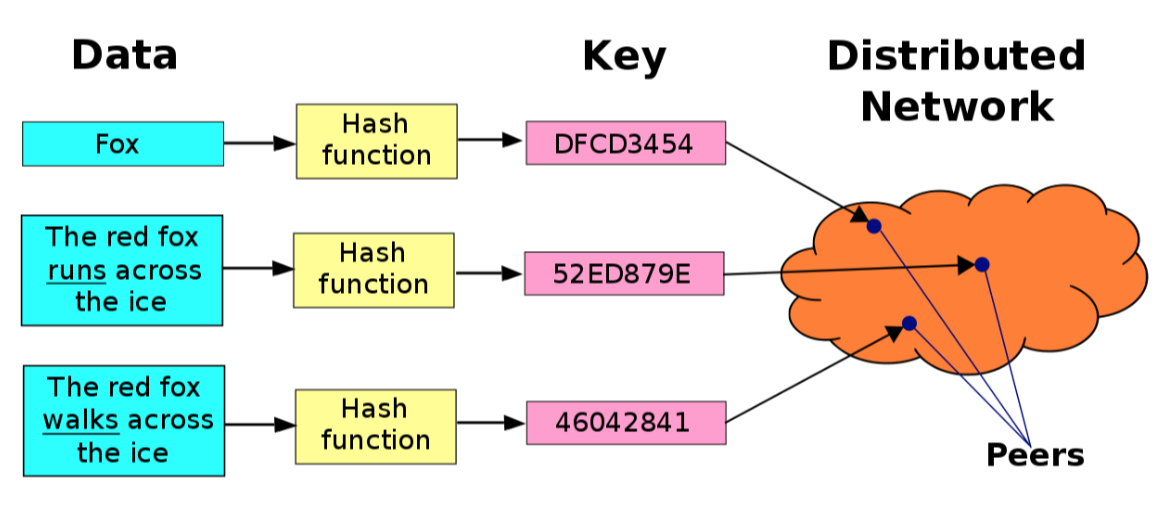
\includegraphics[width=0.7\textwidth]{img/dht}
  \caption{\label{fig:dht} DHT approach}
\end{figure}

\subsubsection{DHT structure}

The structure of a DHT can be decomposed into several main components:
\begin{itemize}
  \item an abstract \textbf{keyspace}, such as the set of 160-bit strings;
  \item a \textbf{keyspace partitioning scheme} splits ownership of this keyspace among the participating nodes;
  \item an \textbf{overlay network} then connects the nodes, allowing them to find the owner of any given key in the keyspace.
\end{itemize}

\begin{figure}[b!]
  \centering
  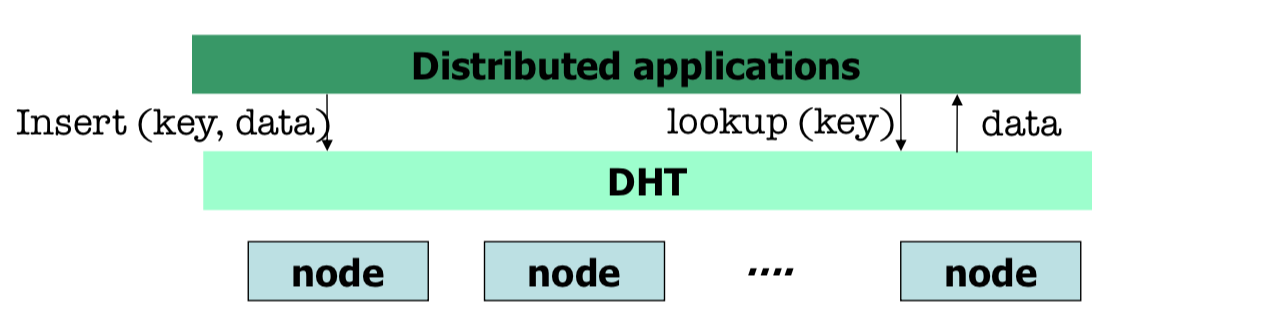
\includegraphics[width=0.8\textwidth]{img/dht-api}
  \caption{\label{fig:dht-api} DHT API}
\end{figure}

\subsubsection{DHT operations}

A typical use of the DHT for storage and retrieval might proceed as follows:
\begin{enumerate}[label=\arabic*.]
  \item to index a file with given filename and data in the DHT, the SHA-1 hash of filename is generated, producing a 160-bit key $k$, and a message \texttt{insert(k, data)} is sent to a node participating in the DHT.
  \item the message is forwarded from node to node through the overlay network until it reaches the single node responsible for key $k$ as specified by the keyspace partitioning. That node then stores the key and the data.
  \item any other client can then retrieve the contents of the file by again hashing filename to produce $k$ and asking a DHT node to find the data associated with $k$ with a message \texttt{lookup(k)}.
  \item the message will again be routed through the overlay to the node responsible for $k$, which will reply with the stored data.
\end{enumerate}

\subsubsection{DHT properties}

DHTs characteristically emphasize the following properties:
\begin{itemize}
  \item \textit{Autonomy and decentralization}: the nodes collectively form the system without any central coordination.
  \item \textit{Fault tolerance}: the system should be reliable even with nodes continuously joining, leaving, and failing.
  \item \textit{Scalability}: the system should function efficiently even with thousands or millions of nodes.
  \item \textit{Load Balancing}: the hash function should evenly distribute keys to nodes.
  \item \textit{Anonimity}: can be achieved by special routing overlay networks that hide the physical location of each node from other participants.
\end{itemize}

\subsection{Pastry}
\textit{Pastry} is a robust, self-organizing peer-to-peer overlay network for DHT. The key-value pairs are stored in a \textbf{redundant} peer-to-peer network of connected hosts. The protocol is bootstrapped by supplying it with the IP address of a peer already in the network and from then on via the \textbf{routing table} which is dynamically built and repaired. Because of its redundant and decentralized nature, there is no single point of failure and any single node can leave the network at any time without warning and with little or no chance of data loss.

\subsubsection{Design}
The topology of the hash table's key-space is \textbf{circular}. NodeIds and keys are 128-bit unsigned integer (in base $2^b$) representing position in the circular space. NodeIds are chosen randomly and uniformly, so peers who are adjacent in nodeId are geographically diverse. Unique nodeIds are assigned when nodes join the system, based on a secure hash of the node’s IP address. Key are stored in the node with nodeId numerically closest to the key, among all live Pastry nodes.

\subsubsection{Routing}
Given a message and a key, Pastry reliably routes the message to the node with the nodeId that is numerically closest to the key. Assuming a network consisting of $N$ nodes, Pastry can route to any node in less than $\ceil{\log_{2^b}N}$ steps on average ($b$ is a configuration parameter with typical value 4). With concurrent node failures, eventual delivery is guaranteed, unless $l/2$ or more nodes with \textit{adjacent} nodeIds fail simultaneously ($l$ is an even integer parameter with typical value 16). The tables required in each Pastry node have only $(2^b - 1) * \ceil{\log_{2^b}N} + l$ entries, where each entry maps a nodeId to the associated node’s IP address.

\paragraph{Prefix routing}
NodeIds and keys are thought of as a sequence of digits with base $2^b$, this for making the routing table more compact. A node's routing table is organized into $\ceil{\log_{2^b}N}$ rows with $2^b - 1$ entries each. The $2^b - 1$ entries in row $n$ each refer to a node whose nodeId matches the present node's nodeId in the first $n$ digits, but whose $n + 1$th digit has one of the $2^b - 1$ possible values other than the $n + 1$th digit in the present node's ID. Each entry in the routing table refers to one of the potentially many nodes whose nodeId have the appropriate prefix. Among such nodes, the one closest to the present node (according to a scalar \textit{proximity metric}, such as the round trip time) is chosen. Figure~\ref{fig:routing-table-1} shows a possible routing table of node with nodeId $65a1x$ and Figure~\ref{fig:routing-table-2} a possible routing table of node with nodeId $10233102$. In the latter, we may notice that the last rows are not completely filled or even empty.

\begin{figure}[t]
  \centering
  
\end{figure}

\begin{figure}[t]
      \centering
      \begin{subfigure}{.45\textwidth}
        \centering
        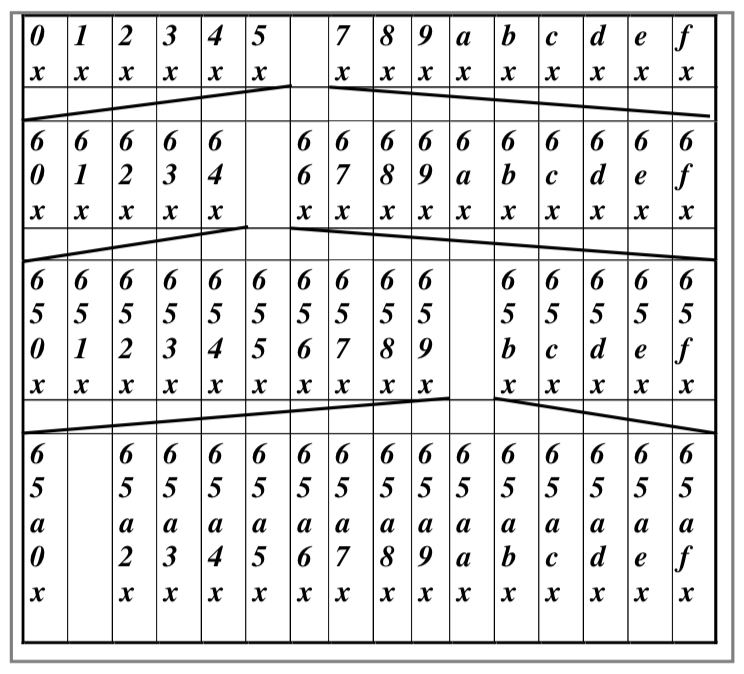
\includegraphics[width=0.8\textwidth]{img/routing-table-1}
        \caption{\label{fig:routing-table-1}Routing table of a Pastry node with nodeId $65a1x$, $b=4$. Digits are in base 16, $x$ represents an arbitrary suffix.}
      \end{subfigure}\hfill%
      \begin{subfigure}{.45\textwidth}
        \centering
        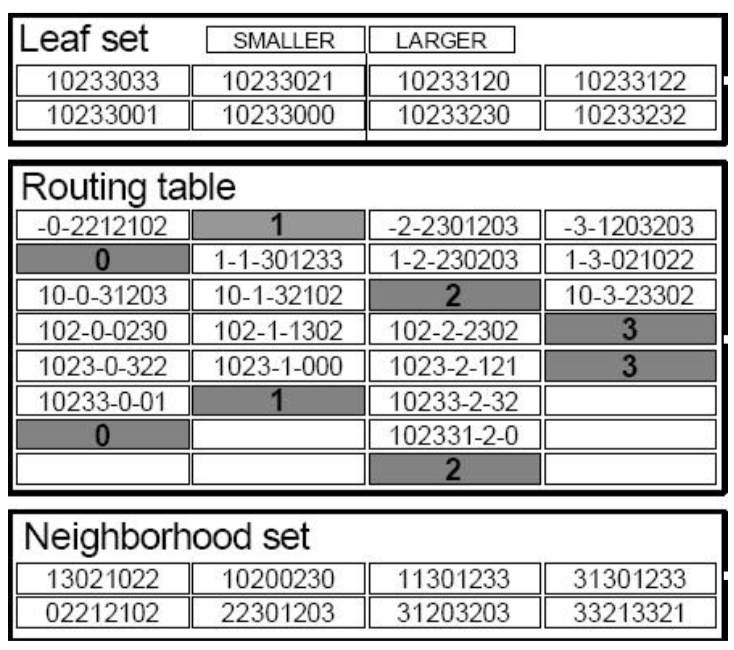
\includegraphics[width=0.8\textwidth]{img/routing-table-2}
        \caption{\label{fig:routing-table-2}Routing table of a Pastry node with nodeId $10233102$, $b=2$, $l=8$. Digits are in base 4.}
      \end{subfigure}
      \caption{Pastry routing table}
    \end{figure}

In addition to the routing table, each node maintains IP addresses for the nodes in its \textit{leaf set}, i.e., the set of nodes with the $l/2$ numerically closest larger nodeIds, and the $l/2$ nodes with numerically closest smaller nodesIDs, relative to the present node's nodeId.

\begin{figure}[b]
  \centering
  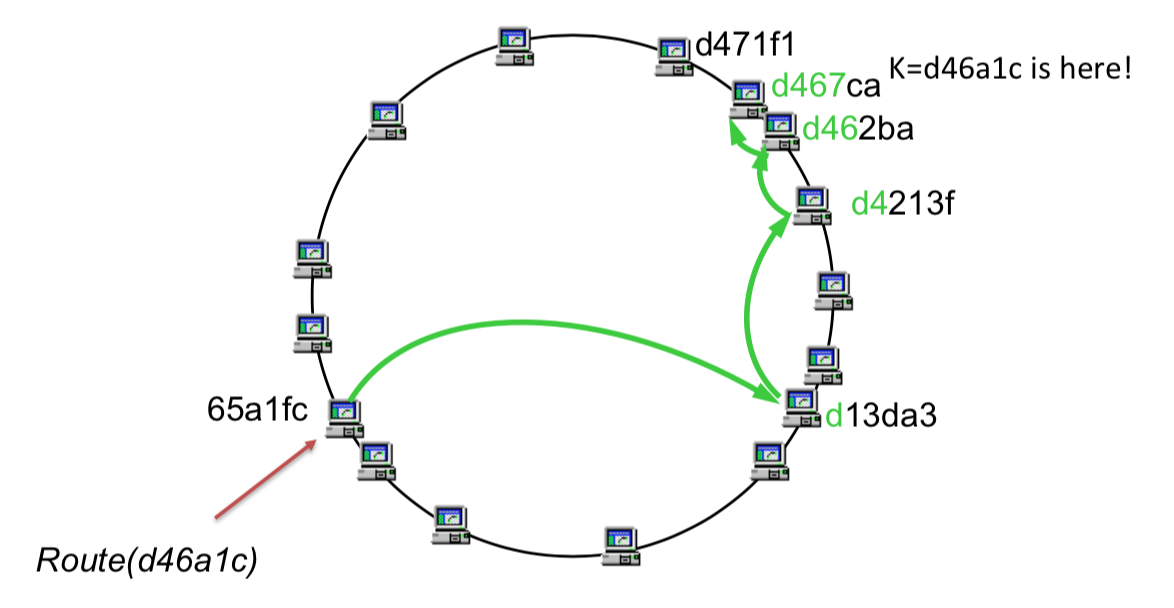
\includegraphics[width=0.6\textwidth]{img/routing-step}
  \caption{\label{fig:routing-step} Routing a message from node $65a1fc$ with key $d46a1c$.}
\end{figure}

\paragraph{Routing step}
Figure~\ref{fig:routing-step} shows the path of an example message.
\begin{enumerate}[label=\arabic*.]
  \item Seek the routing table and forward the message to a node whose nodeId shares with the key a prefix that is at least one digit longer than the prefix that the key shares with the current nodeId.
  \item If no such node is found in the routing table, check the leaf set and forward the message to a node whose nodeId shares a prefix with the key as long as the current node, but is numerically closer to the key than the current nodeId.
  \item If such node does not exist in the leaf set, the key is stored in the current node (unless the $l/2$ adjacent nodes in the leaf set have failed concurrently).
\end{enumerate}

\subsubsection{Locality}
Pastry’s locality describes the properties of Pastry’s routes with respect to the proximity metric. The proximity metric is a scalar value that reflects the “distance” between any pair of nodes, such as the round trip time. It is assumed that a function exists that allows each Pastry node to determine the “distance” between itself and a node with a given IP address. Two main property are discussed in the following:
\begin{itemize}
  \item \textit{short routes} property concerns the total distance, in terms of proximity metric, that messages travel along Pastry routes. Simulations show that the average distance traveled by a message is between 1.59 and 2.2 times the distance between the source and destination in the underlying Internet.
  \item \textit{route convergence} property is concerned with the distance traveled by the two messages sent to the same key before their routes converge. Simulations show that the average distance traveled by each of the two messages before their routes converge is approximately equal to the distance between their respective source nodes.
\end{itemize}

\subsubsection{Node addition}
An arriving node with the newly chosen nodeId $X$ can initialize its state by:
\begin{enumerate}
  \item contacting a \textbf{known} nearby node $A$ (according to the proximity metric) and asking $A$ to route a \textit{join} message using $X$ as the key.
  \item The message is routed to the existing node $Z$ with nodeId numerically closest to $X$.
  \item $X$ then obtains the \textit{leaf set} form $Z$ and the i-th row of the routing table from the i-th node encountered along the route from $A$ to $Z$.
  \item $X$ notifies nodes to update their states.
\end{enumerate}

\subsubsection{Node failure}
To handle node failures, neighboring nodes in the nodeId space (which are aware of each other by virtue of being in each other’s leaf set) periodically exchange keep-alive messages. If a node is unresponsive for a period $T$, it is presumed failed. All members of the failed node’s leaf set are then notified and they update their leaf sets. Since the leaf sets of nodes with adjacent nodeIds overlap, this update is trivial. A recovering node contacts the nodes in its last known leaf set, obtains their current leaf sets, updates its own leaf set and then notifies the members of its new leaf set of its presence. Routing table entries that refer to failed nodes are repaired lazily.

\subsection{Scribe}
Scribe is a scalable application-level multicast infrastructure built on top of Pastry. Any Scribe node may create a \textit{group}; other nodes can then join the group, or multicast messages to all members of the group (provided they have the appropriate credentials). Scribe provides best-effort delivery of multicast messages, and specifies no particular delivery order.

Scribe uses Pastry to manage group creation, group joining and to build a per-group multicast tree used to disseminate the messages multicast in the group. Pastry and Scribe are fully decentralized: all decisions are based on local information, and each node has identical capabilities.

Scribe offers a simple API to its applications to which credentials must be provided:
\begin{itemize}
	\item \texttt{create(credentials, groupId)} creates a group with groupId. 
	\item \texttt{join(credentials, groupId, messageHandler)} causes the local node to join the group with groupId. All subsequently received multicast messages for that group are passed to the specified message handler.
	\item \texttt{leave(credentials, groupId)} causes the local node to leave the group with groupId.
	\item \texttt{multicast(credentials, groupId, message)} causes the message to be multicast within the group with groupId.
\end{itemize}

\subsubsection{Implementation}

A Scribe system consists of a network of Pastry nodes, where each node runs the Scribe application software. The Scribe software on each node provides the \textit{forward} and \textit{deliver} methods, which are invoked by Pastry whenever a Scribe message arrives.

Each group has a unique \textit{groupId}. The Scribe node with a nodeId numerically closest to the groupId acts as the \textit{rendez-vous point} for the associated group. The rendez-vous point is the root of the multicast tree created for the group.

To create a group, a Scribe node asks Pastry to route a \texttt{CREATE} message using the groupId as the key (e.g. \texttt{route(CREATE,groupId)}). Pastry delivers this message to the node with the nodeId numerically closest to groupId. The Scribe deliver method adds the group to the list of groups it already knows about. It also checks the credentials to ensure that the group can be created, and stores the credentials. This Scribe node becomes the rendez-vous point for the group.
The groupId is the hash of the group’s textual name concatenated with its creator’s name. The hash is computed using a collision resistant hash function (e.g. SHA-1), which ensures a uniform distribution of groupIds. Since Pastry nodeIds are also uniformly distributed, this ensures an even distribution of groups across Pastry nodes.

\subsubsection{Subscription}

Scribe creates a multicast tree, rooted at the rendez-vous point, to disseminate the multicast messages in the group. The multicast tree is created using a scheme similar to reverse path forwarding. The tree is formed by joining the Pastry routes from each group member to the rendez-vous point.

Figure~\ref{fig:scribe} illustrates the group joining mechanism. We assume that there is a group with groupId 1100 whose rendez-vous point is the node with the same identifier. The node with nodeId 0111 is joining this group. In this example, Pastry routes the \texttt{JOIN} message to node 1001; then the message from 1001 is routed to 1101; finally, the message from 1101 arrives at 1100. This route is indicated by the solid arrows.


\begin{figure}[t!]
  \centering
  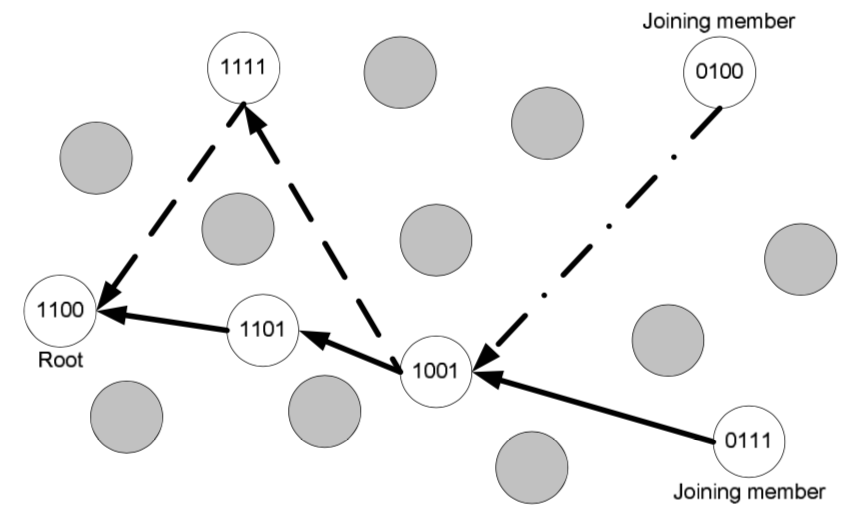
\includegraphics[width=0.5\textwidth]{img/scribe}
  \caption{\label{fig:scribe} Multicast tree creation}
\end{figure}

\subsubsection{Multicast message dissemination}

Multicast sources use Pastry to locate the rendez-vous point of a group: they route to the rendez-vous point (e.g. \texttt{route(MULTICAST, groupId)}), and ask it to return its IP address.
Multicast messages are disseminated from the rendez-vous point along the multicast tree. There is a single multicast tree for each group.

\subsubsection{Repairing the multicast tree}

Periodically, each non-leaf node in the tree sends a heartbeat message to its children. Multicast messages serve as an implicit heartbeat signal avoiding the need for explicit heartbeat messages in many cases. A child suspects that its parent is faulty when it fails to receive heartbeat messages. Upon detection of the failure of its parent, a node calls Pastry to route a \texttt{JOIN} message to the group’s identifier. Pastry will route the message to a new parent, thus repairing the multicast tree.
For example, in Figure~\ref{fig:scribe}, consider the failure of node 1101. Node 1001 detects the failure of 1101 and uses Pastry to route a \texttt{JOIN} message towards the root through an alternative route (indicated by the dashed arrows). The message reaches node 1111 who sends a JOIN message towards the root.

\section{Using Humans as Sensors}
The advent of online social networks, such as Twitter, where humans volunteer free information at scale about the physical world, begs the question of whether or not they can be leveraged as a category of sensor networks. \textit{Mobile crowdsensing} is the process of collecting these information with the aim of inferring any knowledge of common interest.
There exist two types of mobile crowdsensing:
\begin{itemize}
	\item \textit{participatory}: where the user voluntarily participate in contributing information and are aware of doing it;
	\item \textit{opportunistic}: where the data in sensed, collected and shared automatically without user intervention and in some cases, even without the user's explicit knowledge.
\end{itemize}

Among them we are interested in participatory sensing, where the user report the observed physical environment that is external to the (human) sensor. In this case, the physical environment has a unique state, leading to a unique \textit{ground truth}, according to which these descriptions are either true or false. Hence, observation can be viewed as \textit{binary claims}. The sensing problem is to determine which claims are correct, given that the \textit{reliability} of human sensors is generally unknown a priori and the \textit{provenance} of reported observations is \textit{uncertain} (i.e., individuals may report observations made by others as their own).

\subsection{Issues}

We model human participants as (i) \textit{sources of unknown reliability} generating (ii) \textit{binary measurements} of (iii) \textit{uncertain provenance}.

\begin{enumerate}[label=(\roman*)]
	\item \textit{Unknown reliability}: unlike physical sensors, we do not, in general, know the reliability of human observers. The reported physical fact is not accurate and much broader since it can be modified by the human perspective. Moreover different individuals has different reliability, expressed as the probability of producing true claims.
	\item \textit{Binary observations}: Since the reported observations can be aither be true or false, claims can be thought of as measurements of different \textit{binary variables}.
	\item \textit{Uncertain provenance}: it is not unusual for a person to report observations they received from others as if they were his/her own. Such rumor spreading behavior has no analogy in correctly functioning physical sensors. We call this problem one of uncertain data provenance because when Bob tweets that “Main Street is flooded”, even if we authenticate Bob as the actual source of the tweet, we do not know if Bob truely observed that first-hand or heard it from Sally. From a sensing perspective, this means that errors in “measurements” across “sensors” may be non-independent, as one erroneous observation may be propagated by other sources without being verified.
\end{enumerate}

\subsection{A solution architecture}

To enable reconstruction of ground truth information from data reported by human sources, we need to (i) collect unformatted data from the “sensor network”, (ii) structure the data for analysis, (iii) understand how sources are related, and (iv) use this collective information to estimate the probability of correctness of individual observations.

\subsubsection{Data collection}
Data is collected from Twitter through a long-standing query via the exported Twitter API to match given keywords and an indicated geographic region on a map.

\subsubsection{Data structuring}
Next, we need to determine the internal consistency in reported observations. For this reason, observations are clustered based on a \textit{distance function}. This function, \texttt{distance(t1,t2)}, takes two reported observations, $t1$ and $t2$, as input and returns a measure of similarity between them, represented by a logical distance. The more dissimilar the observations, the larger the distance. In the case of data collection from Twitter, we regard individual tweets as individual observations, and borrow from natural language processing literature a \textit{cosine similarity function} that returns a measure of similarity based on the number of matching tokens in the two inputs:

$$ similarity = \cos \theta = \frac{A \cdot B}{||A||\ ||B||} $$

where $A$ and $B$ are vectors of token occurance in tweets.

As distances are computed, the set of input observations is transformed to a graph where vertices are individual observations and links represent similarity among them. We then cluster the graph, causing similar observations to be clustered together. We call each such cluster a \textit{claim}. Hence, the claim represents a piece of information that \textit{several} sources reported.

We can now construct a \textbf{source-claim graph}, \textit{SC}, in which each source, $S_i$, is connected to all claims they made (i.e., clusters they contributed to), and each claim, $C_j$ , is connected to all sources who espoused it (i.e., all sources of tweets in the corresponding cluster). We say that $S_iC_j = 1$ if source $S_i$ makes claim $C_j$. Each claim can either be true or false. The claim is true if it is consistent with ground truth in the physical world. Otherwise, it is false.

\subsubsection{Sources relationship}
Next, we need to account for uncertain provenance. Sources may have reported either their own observations or observations they heard from others. We assume the existence of a latent \textbf{social information dissemination graph}, \textit{SD}, that estimates how information might propagate from one person to another:

\begin{itemize}
	\item \textit{Epidemic Cascade network (EC)}: each distinct observation is modeled as a cascade and the time of contagion of a source describes when the source mentioned this observation.
	\item \textit{Follower-Followee network (FF)}: A directed link $(S_i, S_k)$ exists in the social graph from source $S_i$ to source $S_k$ if $S_k$ is a follower of $S_i$.
	\item \textit{Re-Tweeting network (RT)}: a directed link $(S_i, S_k)$ exists in the social graph if source $S_k$ retweets some tweets from source $S_i$.
	\item \textit{RT+FF network}: a directed link $(S_i, S_k)$ exists when either $S_k$ follows $S_i$ or $S_k$ retweets what $S_i$ said.
\end{itemize}

\subsubsection{Estimation problem}

Tweets are analyzed using a sliding window with size $N$. Now we can follow two schemes:

\begin{itemize}
	\item \textit{Voting}: claims with more support are more believable. For each $C_j$, where $1 \le j \le N$, count all $S_i$, where $S_iC_j = 1$. Unfortunately, it is suboptimal for two reasons. First, different sources have different degrees of reliability. Hence, their “votes” do not have the same weight. Second, sources may not be independent. When a source simply repeats what they heard from others, their “vote” does not add to the credibility of the claim.
	
	\item \textit{Likelihood estimation}: given graphs $SC$ and $SD$ what is the likelihood that claim $C_j$ is true, for each $j$? Formally, we compute:

	$$ \forall j, 1 \le j \le N : P(C_j = 1 | SC, SD) $$

	where $P(C_j = 1|SC, SD)$ is the conditional probability that $C_j$ is true given $SC$ and $SD$.
\end{itemize}

\subsubsection{Maximum Likelihood (ML) Estimation}

Let $m$ be the total number of sources in our system from which we have data. Let us describe each source (i.e., “sensor”), $S_i$, $1 \le i \le m$, by two parameters, neither of which are known in advance:
\begin{itemize}
	\item the odds of true positives, $a_i = P(S_iC_j = 1|C_j = 1)$
	\item the odds of false positives, $b_i = P(S_iC_j = 1|C_j = 0)$
\end{itemize}
Let us also denote by $d$ the unknown expected ratio of correct claims in the system, $d = P(C_j = 1)$. Let us now define the vector $\theta$ to be the vector of the above unknowns:

$$ \theta = [a_1 \dots a_m b_1 \dots b_m d] $$

A maximum likelihood estimator finds the values of the unknowns that maximize the probability of observations, $SC$, given the social network $SD$. Hence, we would like to find $\theta$ that maximizes $P(SC|SD,\theta)$. The probability $P(SC|SD,\theta)$ depends on which claims are true and which are false. Let us therefore introduce the vector $Z$ where element $z_j = 1$ if $C_j$ is true and zero otherwise. Using the total probability theorem, we can now rewrite the expression we want to maximize, namely $P(SC|SD,\theta)$, as follows:

$$ P(SC|SD,\theta) = \sum_z P(SC,z|SD,\theta) $$

The solution of the maximization of MLE can be found using algorithms described in the literature, incorporating the role of uncertain provenance into the maximum likelihood estimation algorithm. Let us divide the source claim graph $SC$ into subsets, $SC_j$, one per claim $C_j$. The subset describes which sources espoused the claim and which did not.

We can define $Z(n,j)$ as the conditional probability of claim $C_j$ to be true given the observed source claim subgraph $SC_j$ and current estimation on $\theta$:

$$ Z(n,j) = p(z_j = 1 | SC_j, \theta^{(n)}) $$

In general, the sources that make these observations may not be independent since they may be connected in the social network leading to a possibility that one repeated the observation of another. Let $p_{ik} = P(S_iC_j|S_kC_j)$ be the probability that source $S_i$ makes claim $C_j$ given that his parent $S_k$ (in the social dissemination network) makes that claim. We call $p_{ik}$ a \textit{repeat ratio} and can approximately compute it from graph $SC$, for pairs of nodes connected in graph $SD$, as follows:

$$ p_{ik} = \frac{\text{number of times } S_i \text{ and } S_k \text{ make same claim}}{\text{number of claims } S_k \text{ makes}} $$

\begin{figure}[t!]
  \centering
  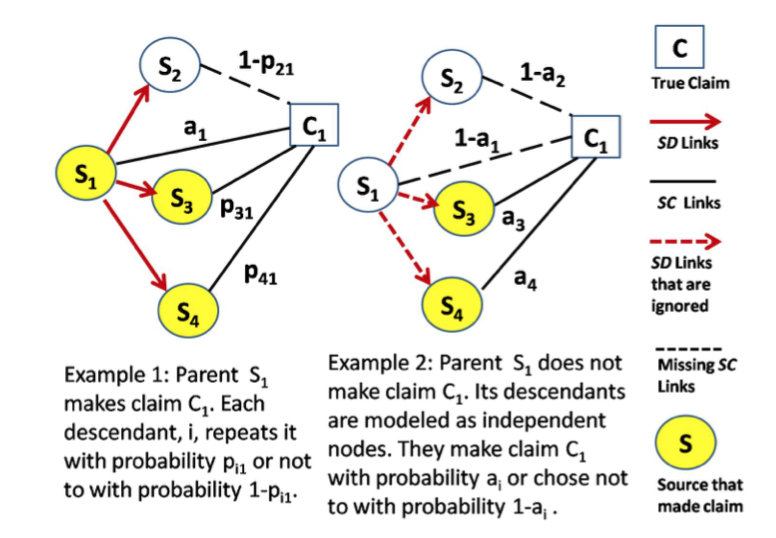
\includegraphics[width=0.5\textwidth]{img/mle}
  \caption{\label{fig:mle} Example}
\end{figure}

Considering the example in Figure~\ref{fig:mle}, the intuition is that if the parent does not make the claim, then the children act as if they are independent sources. If the parent makes the claim, then each child repeats it with a given repeat probability.

The algorithm takes as input the source claim graph $SC$ from social sensing data and the source dissemination graph $SD$ estimated from social network, and the output is the maximum likelihood estimation of source reliability and claim correctness. In particular, given the source claim graph $SC$, the algorithm begins by initializing the parameter $\theta$ with random values between 0 and 1. We also estimate the dependent ratio of each non-independent source (i.e., $p_{ik}$) from the source disseminate graph SD. The algorithm then iterates until $\theta$ converges. Finally, we can decide whether each claim $C_j$ is true or not based on the converged value of $Z(n,j)$. Specifically $C_j$ is true if $Z(n,j) \ge 0.5$ and false otherwise. 

\subsection{Evaluation}

Figure~\ref{fig:mle-eval} shows the result for the hurricane Sandy trace. To compare these algorithms, we implemented them inside Apollo. We observe that the Apollo-social generally outperformed the regular EM schemes in providing more true claims and suppressing the unconfirmed claims. This is achieved by incorporating the source dependency into the analytical framework of expectation maximization to better handle non-independent sources and their claims. The performance advantage of Apollo-social compared to regular EM is significant (nearly 20\%) if we use the combined social network information (i.e, RT+FF social network) constructed from follower-followee and retweet relationship between users. We observed that the performance of the Apollo-social using Epidemic Cascades (EC) to estimate the social network is between Apollo-social using RT and FF social network. The reason is the RT social network is generated from the retweet relationship from current data interval and is very dynamic to reflect current source dependency and while FF social network is generated from the follower-followee relationship independently from the data traces and is relatively static. The dynamics of source dependency of EC social network is between RT and FF social network.

\begin{figure}[H]
  \centering
  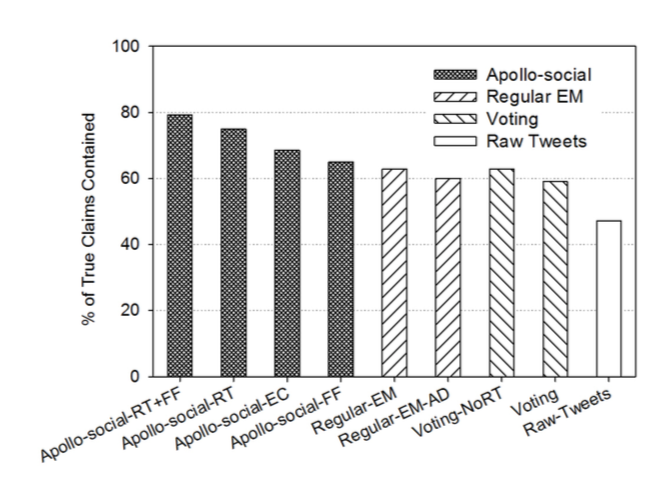
\includegraphics[width=0.5\textwidth]{img/mle-eval}
  \caption{\label{fig:mle-eval} Evaluation of Hurricane Sandy Trace}
\end{figure}

















\end{document}